\chapter{HASIL DAN PEMBAHASAN}

\section{Pembangunan \textit{Virtual Machine} (VM) di DigitalOcean}
Pembangunan \textit{virtual machine} pada penelitian ini adalah hal yang krusial karena semua komputasi akan dijalankan pada \textit{platform cloud} DigitalOcean. VM yang sudah berhasil terinisiasi akan terlihat seperti pada Gambar \ref{fig:00-tampilan-digitalocean}.

\begin{figure}[h]
    \centering
    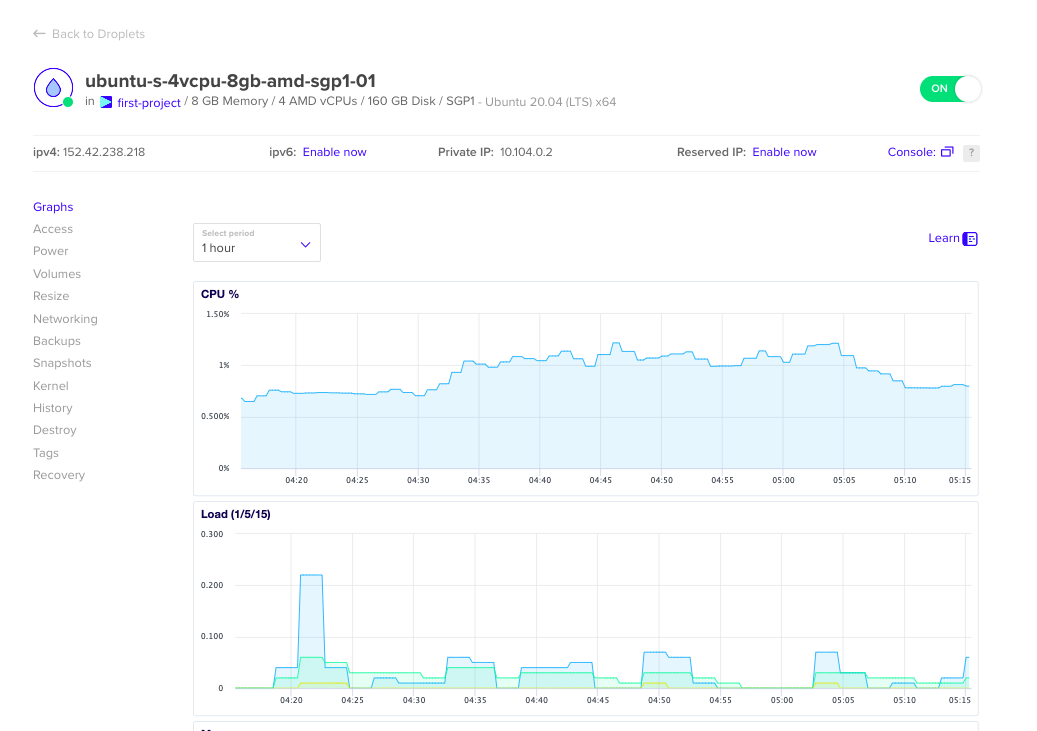
\includegraphics[width=1\textwidth]{figures/ch04/00-tampilan-digitalocean}
    \caption{Tampilan Dasbor VM DigitalOcean}
    \label{fig:00-tampilan-digitalocean}
\end{figure}


\section{Pemasangan dan Konfigurasi Perangkat Lunak}
Penelitian ini membandingkan kinerja Hadoop dan Spark pada \textit{platform cloud} DigitalOcean menggunakan alat pengujian data besar yang bernama HiBench pada lingkup \textit{Micro Benchmarks}, yaitu \textit{Word Count} dan \textit{Sort} dengan data masukan berupa teks yang dibuat oleh \textit{data generation} pada tahap persiapan. 

Sebelum memulai eksperimen, serangkaian pemeriksaan dilakukan untuk memastikan bahwa semua perangkat lunak yang terlibat berfungsi dengan baik. Tahapan ini penting untuk menjamin validitas hasil penelitian. Berikut adalah pemeriksaan yang dilakukan, yaitu
\begin{enumerate}
	\item \textbf{Pengecekan versi Hadoop}. Versi Hadoop yang digunakan dalam penelitian ini adalah 2.4.0. Verifikasi versi dilakukan melalui perintah \textit{hadoop version}, seperti yang ditunjukkan pada Gambar \ref{fig:versi-hadoop}. 
		\begin{figure}[h]
		    \centering
		    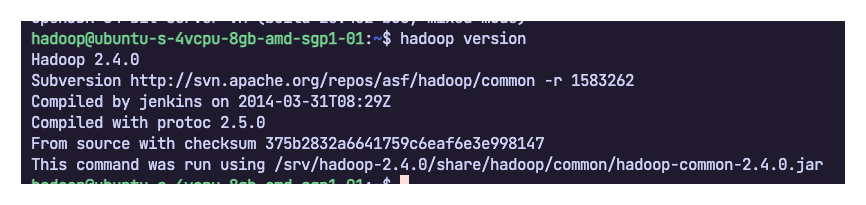
\includegraphics[width=0.9\textwidth]{figures/ch04/versi-hadoop}
		    \caption{Pengecekan Versi Hadoop}
		    \label{fig:versi-hadoop}
		\end{figure}
	\item \textbf{Pengecekan versi Spark}. Versi Spark yang digunakan adalah 2.1.3. Verifikasi dilakukan dengan perintah \textit{spark-submit --version}, seperti yang ditunjukkan pada Gambar \ref{fig:versi-spark}.
		\begin{figure}[h]
		    \centering
		    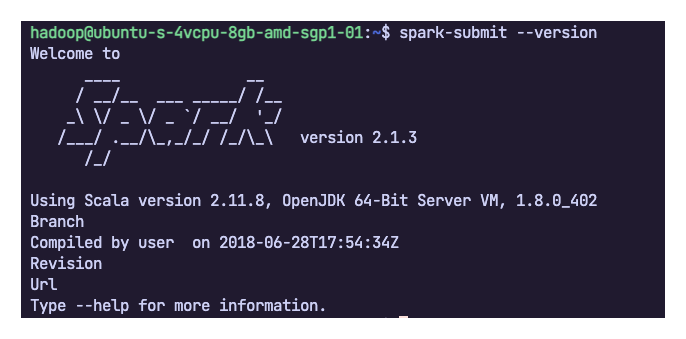
\includegraphics[width=0.85\textwidth]{figures/ch04/versi-spark}
		    \caption{Pengecekan Versi Spark}
		    \label{fig:versi-spark}
		\end{figure}
	\item \textbf{Pemeriksaan \textit{service} yang berjalan ketika tanpa beban kerja}. Status layanan (\textit{services}) yang berjalan pada komputer diperiksa dalam keadaan tanpa beban kerja (\textit{idle}). Layanan yang diharapkan aktif meliputi: Jps, ResourceManager, DataNode, NodeManager, NameNode, dan SecondaryNameNode. Gambar \ref{fig:service-dasar} menunjukkan hasil pemeriksaan layanan dasar.		
		\begin{figure}[h]
		    \centering
		    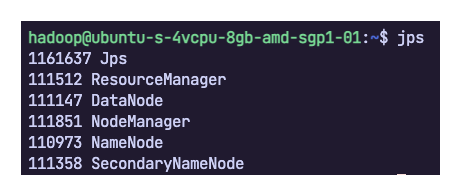
\includegraphics[width=0.8\textwidth]{figures/ch04/service-dasar}
		    \caption{Pengecekan \textit{Service} yang Berjalan (Normal)}
		    \label{fig:service-dasar}
		\end{figure}
	\newpage
	\item \textbf{Pemeriksaan \textit{service} yang berjalan ketika menggunakan Hadoop}. Ketika beban kerja Hadoop dijalankan, layanan tambahan seperti YarnChild, MRAppMaster, dan RunJar  diharapkan aktif, di samping layanan dasar yang telah disebutkan. Gambar \ref{fig:service-hadoop} menunjukkan hasil pemeriksaan layanan saat Hadoop aktif.
		\begin{figure}[h]
		    \centering
		    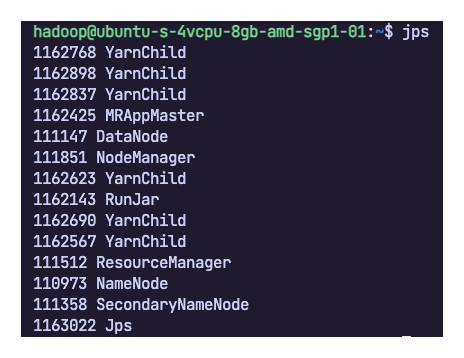
\includegraphics[width=0.7\textwidth]{figures/ch04/service-hadoop}
		    \caption{Pengecekan \textit{Service} yang Berjalan (Hadoop)}
		    \label{fig:service-hadoop}
		\end{figure}
	\item \textbf{Pemeriksaan \textit{service} yang berjalan ketika menggunakan Spark}. Ketika beban kerja Spark dijalankan, layanan seperti CoarseGrainedExecutorBackend, ExecutorLauncher, dan SparkSubmit diharapkan aktif, di samping layanan dasar.  Gambar \ref{fig:service-spark} menunjukkan hasil pemeriksaan layanan saat Spark aktif.
		\begin{figure}[h]
		    \centering
		    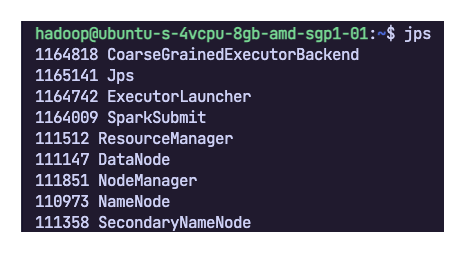
\includegraphics[width=0.8\textwidth]{figures/ch04/service-spark}
		    \caption{Pengecekan \textit{Service} yang Berjalan (Spark)}
		    \label{fig:service-spark}
		\end{figure}
\end{enumerate}

\newpage
\section{Eksperimen}
Selama pengujian, beberapa parameter pada HiBench, Hadoop, dan Spark dikonfigurasi secara tetap untuk menjaga konsistensi dan memungkinkan perbandingan yang adil. Tabel \ref{table:conf-hibench} dan Tabel \ref{table:conf-spark} merangkum konfigurasi parameter yang digunakan.

\begin{table}[h]
\caption{Konfigurasi HiBench}
\label{table:conf-hibench}
\centering
\begin{tabular}{l c p{5cm}} 
\hline
%\multicolumn{1}{c}{\textbf{Nama Parameter}}  & \multicolumn{1}{c}{\textbf{Nilai}} & \multicolumn{1}{c}{\textbf{Keterangan}}  \\ \hline
\textbf{Nama Parameter} & \textbf{Nilai} & \textbf{Keterangan Parameter} \\ \hline
\textit{hibench.default.map.parallelism}     & 8 & \textit{Mapper numbers} (Hadoop), \textit{partition numbers} (Spark)                          \\
\textit{hibench.default.shuffle.parallelism} & 8 & \textit{Reducer numbers}  (Hadoop), \textit{shuffle partition} (Spark)\\ \hline                        
\end{tabular}
\end{table}

\begin{table}[h]
\caption{Konfigurasi Spark}
\label{table:conf-spark}
\centering
\begin{tabular}{l c p{5cm}} 
\hline
\textbf{Nama Parameter} & \textbf{Nilai Parameter} & \textbf{Keterangan Parameter} \\ \hline
\textit{hibench.yarn.executor.num} & 2 & Jumlah \textit{executor} \\
\textit{hibench.yarn.executor.cores} & 4 & Jumlah \textit{core} CPU setiap \textit{executor}\\ 
\textit{spark.executor.memory} & 4 GB & Jumlah memori setiap \textit{executor} \\
\textit{spark.driver.memory} & 4 GB & Jumlah memori tiap \textit{driver} Spark\\ \hline                        
\end{tabular}
\end{table}

Parameter \textit{hibench.default.map.parallelism} memiliki peran yang berbeda pada Hadoop dan Spark. Pada Hadoop, parameter ini menentukan jumlah \textit{mapper}, yaitu proses yang bertanggung jawab untuk memproses data secara paralel pada tahap \textit{Map}. Pada Spark, parameter ini menentukan jumlah partisi data, yaitu unit pemrosesan dasar dalam Spark.

Parameter \textit{hibench.default.shuffle.parallelism} juga memiliki peran yang berbeda pada Hadoop dan Spark. Pada Hadoop, parameter ini menentukan jumlah \textit{Reducer}, yaitu proses yang bertanggung jawab untuk menggabungkan hasil dari tahap \textit{Map}. Pada Spark, parameter ini menentukan jumlah \textit{Shuffle partition}, yaitu jumlah partisi data yang digunakan selama tahap \textit{Shuffle}, yaitu proses pengocokan dan pengurutan data antara tahap \textit{Map} dan \textit{Reduce}.

%Berikut penjelasan mengenai parameter Spark pada Tabel \ref{table:conf-spark}:
%\begin{enumerate}
%	\item \textbf{hibench.yarn.executor.num}: Parameter ini menentukan jumlah \textit{executor} yang akan dialokasikan untuk aplikasi Spark. \textit{Executor} adalah proses yang berjalan pada node pekerja (\textit{worker node}) di kluster YARN dan bertanggung jawab untuk menjalankan task Spark.
%	\item \textbf{hibench.yarn.executor.cores}: Parameter ini menentukan jumlah core CPU yang dialokasikan untuk setiap \textit{executor}. Semakin banyak core yang dialokasikan, semakin banyak task yang dapat dijalankan secara paralel oleh setiap \textit{executor}.
%	\item \textbf{spark.executor.memory}: Parameter ini menentukan jumlah memori yang dialokasikan untuk setiap \textit{executor}. Memori ini digunakan untuk menyimpan data yang diproses oleh \textit{executor}, seperti RDD dan data yang di-\textit{cache}.
%	\item \textbf{spark.driver.memory}: Parameter ini menentukan jumlah memori yang dialokasikan untuk proses driver Spark. Driver bertanggung jawab untuk mengelola aplikasi Spark, menjadwalkan task, dan mengumpulkan hasil.
%\end{enumerate}

\section{Data Keluaran yang Dihasilkan}

Setiap pengujian akan menghasilkan berkas output berupa data HiBench \textit{Report} dan Dool \textit{System Monitoring}. Data HiBench \textit{Report} akan terlihat seperti pada Gambar \ref{fig:data-hibench-report}. Pada Gambar \ref{fig:data-hibench-report}, terlihat bahwa ekstensi berkasnya \textit{.report} dan terlihat beberapa data seperti jenis beban kerja, aplikasi yang digunakan, besar input data, durasi, dan \textit{throughput}.

\begin{figure}[h]
    \centering
    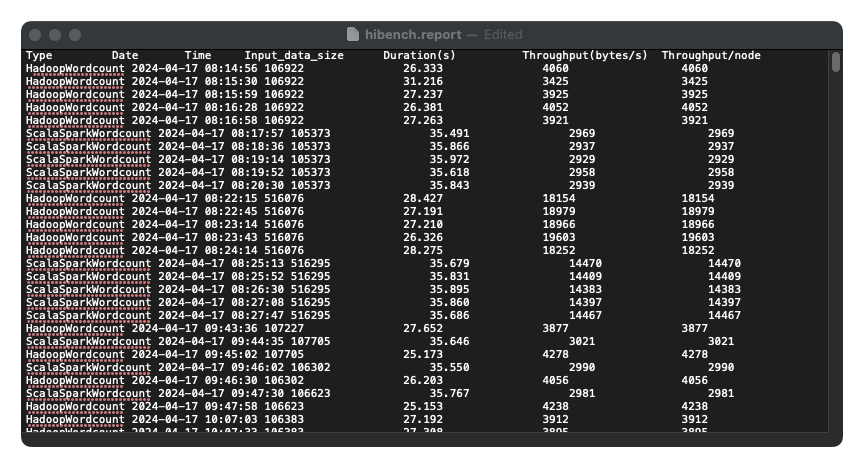
\includegraphics[width=1\textwidth]{figures/ch04/data-hibench}
    \caption{Data HiBench \textit{Report}}
    \label{fig:data-hibench-report}
\end{figure}

Dool, alat monitoring sistem, menghasilkan berkas CSV (\textit{comma-separated value}) untuk setiap perulangan eksperimen. Dengan demikian, terdapat sekitar 240 berkas CSV. Penamaan berkas mengikuti format: [jenis beban kerja]-[ukuran data]-[nomor perulangan]-[aplikasi]. Sebagai contoh, \textit{sort-fivegig-1-hadoop.csv} menunjukkan \textit{data monitoring} untuk beban kerja sort, data masukan 5 GB, perulangan pertama, dan aplikasi Hadoop.

Struktur data Dool, yang ditunjukkan pada Gambar \ref{fig:data-dool-dalam}, mencakup baris \textit{header} (baris 1-4) dan nama kolom (baris 6). Data ini akan dianalisis lebih lanjut untuk mendapatkan \textit{insight} tentang kinerja Hadoop dan Spark.

\begin{landscape}
\begin{figure}[h]
    \centering
    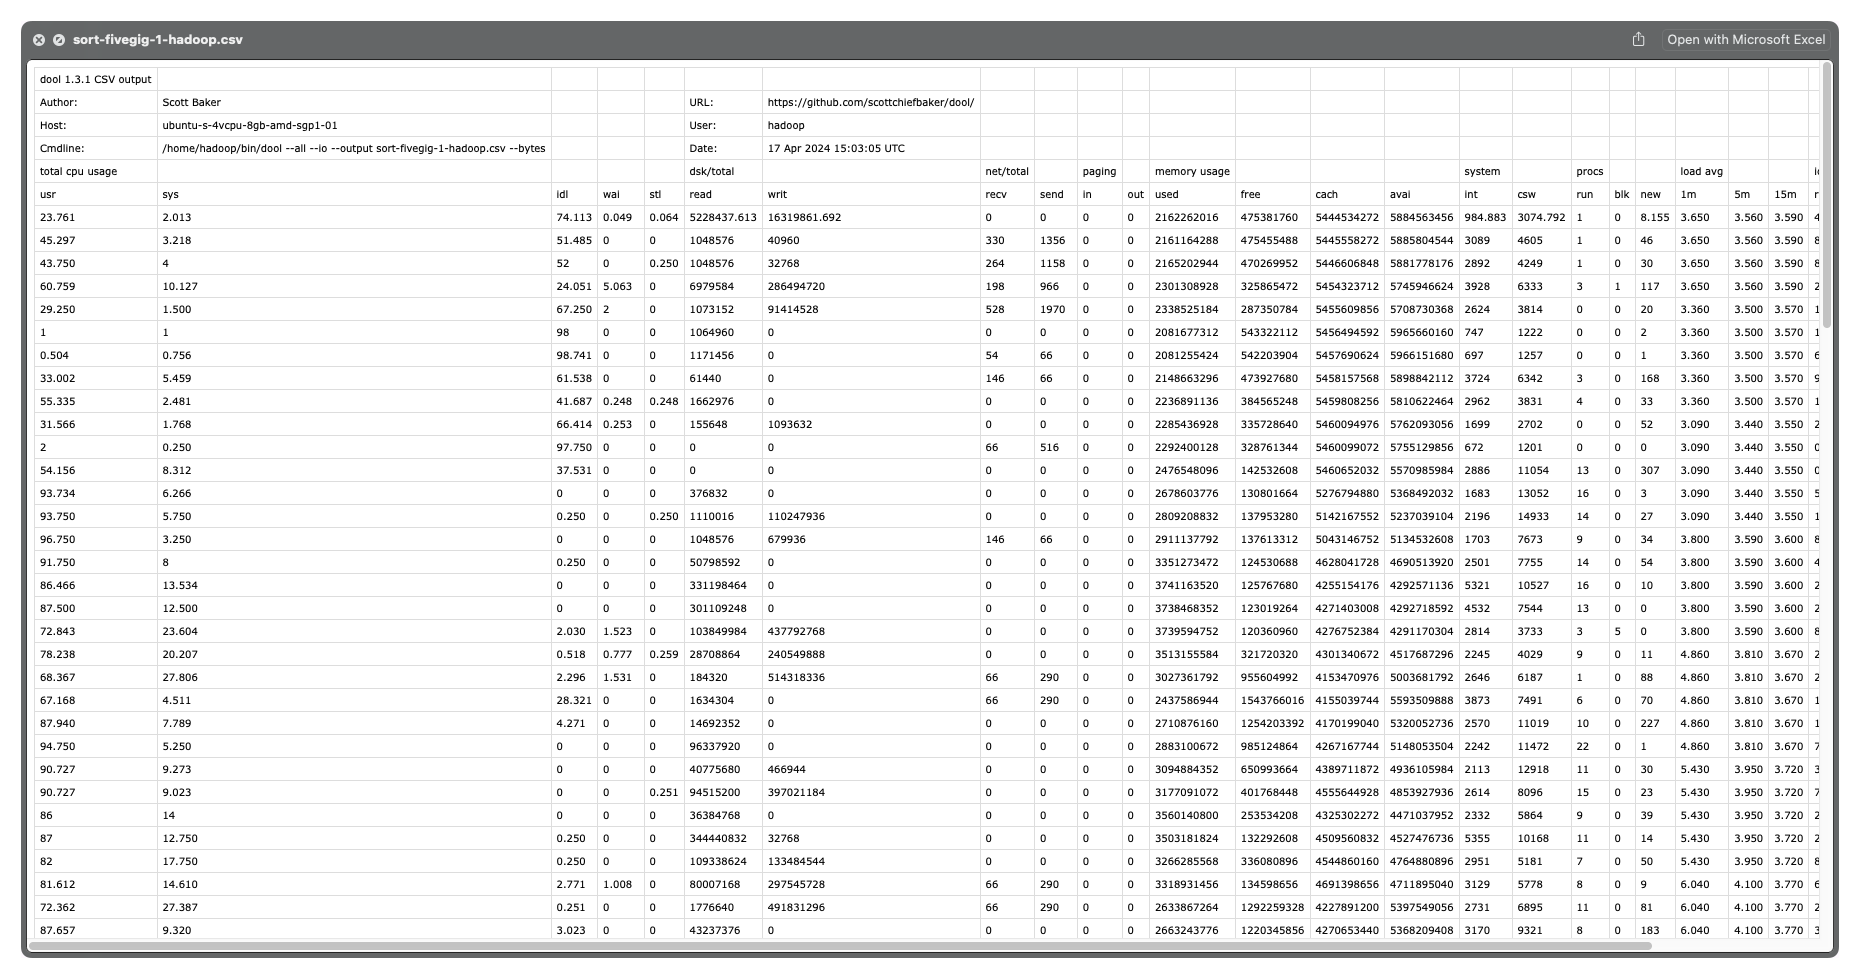
\includegraphics[width=\linewidth, height=0.5\linewidth]{figures/ch04/data-dool-dalam}
    \caption{Contoh Data Dool}
    \label{fig:data-dool-dalam}
\end{figure}
\end{landscape}

\section {Analisis dan Evaluasi Hasil Eksperimen: Kinerja}
\subsection{Persebaran Waktu Eksekusi pada Hadoop dan Spark}

Gambar \ref{fig:lama-waktu-eksekusi-sort} dan Gambar \ref{fig:lama-waktu-eksekusi-wordcount} menyajikan \textit{scatter plot} yang membandingkan performa Hadoop dan Spark dalam dua tugas pemrosesan data yang berbeda, yaitu \textit{sort} dan \textit{word count}. Sumbu x pada kedua gambar menunjukkan variasi ukuran input data, mulai dari 100 KB hingga 15 GB, sementara sumbu y menunjukkan waktu eksekusi dalam detik.

Pada Gambar \ref{fig:lama-waktu-eksekusi-sort}, terlihat bahwa waktu eksekusi Hadoop untuk input data 100 KB hingga 1 GB secara konsisten lebih cepat dibandingkan Spark. Hadoop berada pada rentang waktu 20 hingga 40 detik, sedangkan Spark berada pada rentang waktu 35 hingga 45 detik. Namun, untuk input data sebesar 5 GB, Spark menunjukkan waktu eksekusi yang lebih cepat dibandingkan Hadoop. Spark berada pada rentang 80 hingga 100 detik, sementara Hadoop berada pada rentang 110 hingga 125 detik. Perbedaan performa ini semakin signifikan seiring bertambahnya ukuran data, terutama pada ukuran data 10 GB dan 15 GB. Perbedaan waktu eksekusi antara Hadoop dan Spark semakin jauh pada beban kerja \textit{sort} dengan ukuran data yang lebih besar.

\begin{figure}[h]
    \centering
    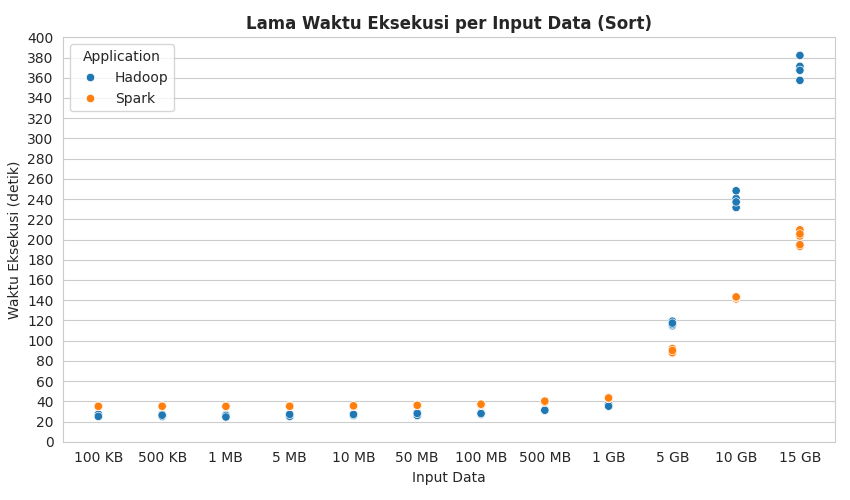
\includegraphics[width=0.8\textwidth]{figures/ch04/1-lama-waktu-eksekusi-sort.png}
    \caption{Persebaran Waktu Eksekusi \textit{Sort} (Hadoop, Spark)}
    \label{fig:lama-waktu-eksekusi-sort}
\end{figure}

Tabel \ref{table:4-sort-dur-table} menunjukkan data yang lebih rinci mengenai durasi waktu eksekusi \textit{sort} untuk Hadoop dan Spark. Berdasarkan tabel tersebut, terlihat bahwa untuk ukuran input data yang kecil hingga menengah, Hadoop relatif lebih cepat daripada Spark. Namun, seiring bertambahnya ukuran input data, Spark menunjukkan performa yang lebih baik dengan waktu eksekusi yang lebih singkat.

\begin{table}[h]
  \centering
  \caption{Statistika Deskriptif Lama Waktu Eksekusi (\textit{Sort})}
  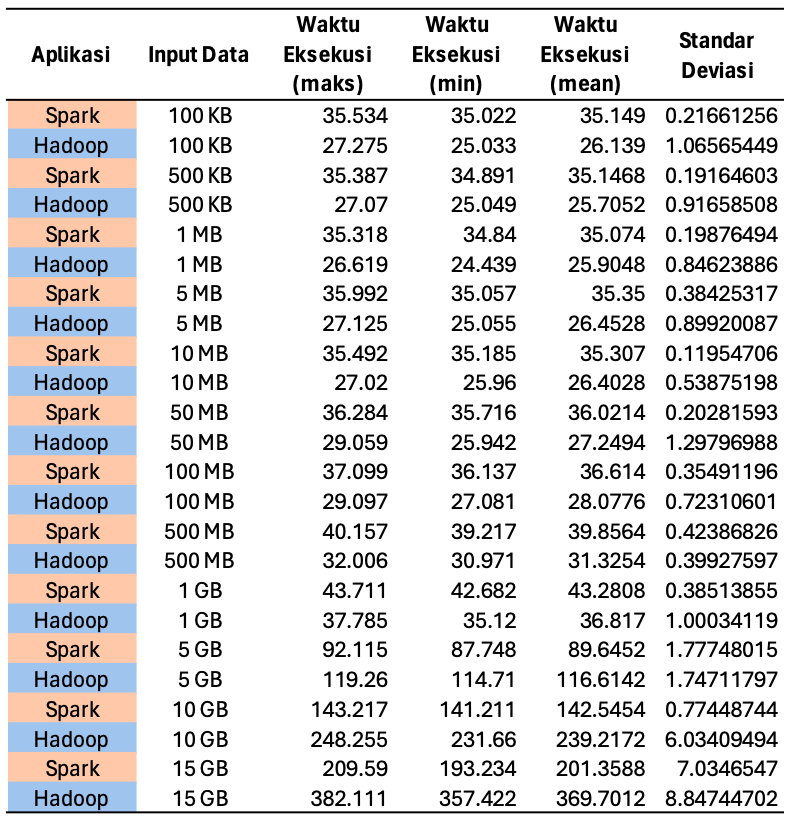
\includegraphics[width=0.6\textwidth]{figures/ch04/4-sort-dur-table}
  \label{table:4-sort-dur-table}
\end{table}

\newpage
Pada Gambar \ref{fig:lama-waktu-eksekusi-wordcount}, Spark menunjukkan performa yang lebih baik dibandingkan Hadoop untuk ukuran input data 500 MB, 1 GB, 5 GB, 10 GB, dan 15 GB pada beban kerja \textit{word count}. Namun, untuk ukuran input data 100 KB hingga 100 MB, Hadoop masih lebih unggul. Waktu eksekusi Hadoop untuk input data 100 KB hingga 100 MB berada pada rentang 20 hingga 40 detik, meskipun perbedaannya tidak signifikan dibandingkan Spark karena titik data Hadoop dan Spark saling berdekatan.

\begin{figure}[h]
    \centering
    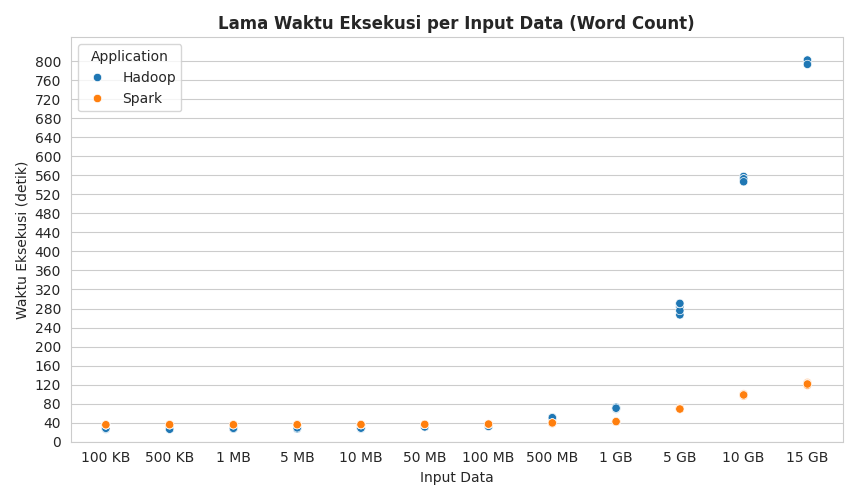
\includegraphics[width=0.8\textwidth]{figures/ch04/1-lama-waktu-eksekusi-wordcount.png}
    \caption{Persebaran Waktu Eksekusi \textit{Word Count} (Hadoop, Spark)}
    \label{fig:lama-waktu-eksekusi-wordcount}
\end{figure}

\newpage
Tabel \ref{table:4-wc-dur-table} menunjukkan data yang lebih rinci mengenai durasi waktu eksekusi \textit{word count} untuk Hadoop dan Spark. Berdasarkan tabel tersebut, terlihat bahwa Hadoop lebih cepat daripada Spark untuk ukuran input data yang kecil hingga menengah yaitu pada 100 KB hingga 100 MB, tetapi Spark lebih cepat untuk ukuran input data yang besar.

\begin{table}[ht]
  \centering
  \caption{Statistika Deskriptif Lama Waktu Eksekusi (\textit{Word Count})}
  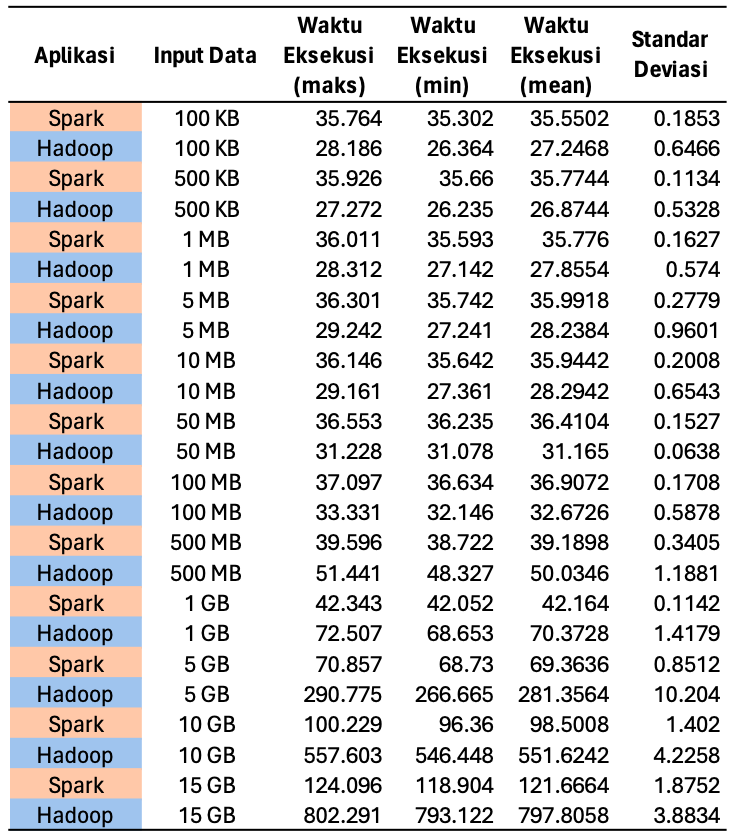
\includegraphics[width=0.6\textwidth]{figures/ch04/4-wc-dur-table}
  \label{table:4-wc-dur-table}
\end{table}

Hasil ini menunjukkan bahwa Spark lebih unggul dan konsisten dibandingkan Hadoop dalam menangani tugas pemrosesan data yang lebih besar, dengan rincian sebagai berikut:
\begin{enumerate}
\item Untuk beban kerja \textit{sort}, Spark lebih unggul mulai dari ukuran input data 5 GB, 10 GB, dan 15 GB.
\item Untuk beban kerja \textit{word count}, Spark lebih unggul mulai dari ukuran input data 500 MB, 1 GB, 5 GB, 10 GB, dan 15 GB.
\end{enumerate}

Secara keseluruhan, Spark menunjukkan kinerja yang lebih baik dalam menangani data berukuran besar, sementara Hadoop lebih efisien untuk data berukuran kecil hingga menengah.

% ----------------------------------------
\subsection {Persebaran \textit{Throughput} pada Hadoop dan Spark}

\textit{Throughput} adalah kecepatan pertukaran data per detik. Kegiatan pertukaran data tersebut terjadi pada \textit{node} yang dipakai dalam komputer komputasi, saat Hadoop maupun Spark memproses data. Oleh karena itu, semakin tinggi nilai \textit{throughput}, semakin sedikit waktu yang dibutuhkan untuk menyelesaikan komputasi. Satuan \textit{throughput} pada penelitian ini adalah MB/s (mega bita per detik).

Gambar di bawah menyajikan \textit{scatter plot} yang membandingkan \textit{throughput} Hadoop dan Spark dalam dua tugas pemrosesan data, yaitu \textit{sort} (Gambar \ref{fig:throughput-sort}) dan \textit{word count} (Gambar \ref{fig:throughput-wordcount}). Sumbu x pada kedua gambar menunjukkan variasi ukuran input data, sedangkan sumbu y menunjukkan \textit{throughput} dalam MB/s.

Pada tugas \textit{sort} (Gambar \ref{fig:throughput-sort}), Spark menunjukkan peningkatan \textit{throughput} yang signifikan seiring dengan bertambahnya ukuran data. Pada ukuran data terbesar (15 GB), Spark mencapai \textit{throughput} sekitar 70 MB/s. Sebaliknya, Hadoop menunjukkan peningkatan \textit{throughput} yang lebih lambat dan hanya mencapai sekitar 40 MB/s pada ukuran data yang sama. Hal ini menunjukkan bahwa Spark mampu melakukan pertukaran data yang lebih besar daripada Hadoop.

\begin{figure}[h]
    \centering
    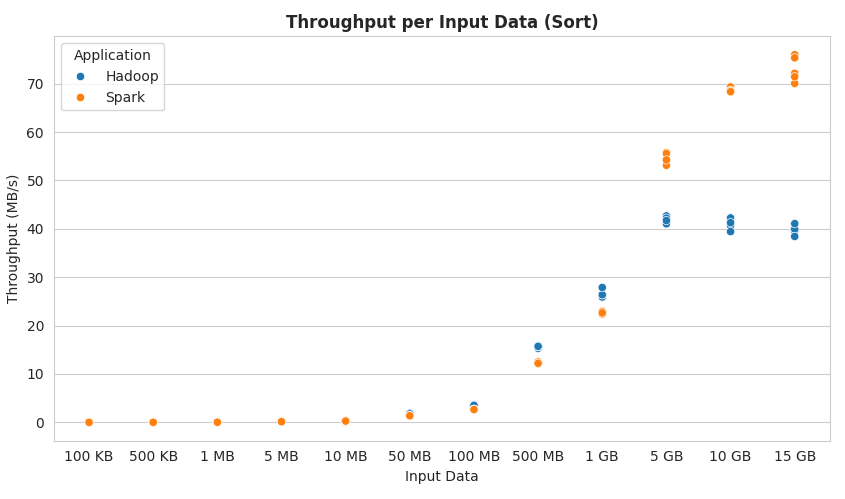
\includegraphics[width=0.8\textwidth]{figures/ch04/1-throughput-sort.png}
    \caption{Persebaran \textit{Throughput Sort} (Hadoop, Spark)}
    \label{fig:throughput-sort}
\end{figure}

Tabel \ref{table:4-sort-th-table} menunjukkan data yang lebih rinci mengenai \textit{throughput} \textit{sort} untuk Hadoop dan Spark. Berdasarkan tabel tersebut, terlihat bahwa Hadoop memiliki \textit{throughput} yang lebih rendah dibandingkan Spark, terutama pada ukuran data yang lebih besar.
Perbedaan kinerja ini dapat dilihat dari kolom "Throughput (maks)" dan "Throughput (min)". Misalnya, untuk input data 100 KB, Hadoop memiliki \textit{throughput} maksimum 0.00403214 MB/s, sedangkan Spark memiliki \textit{throughput} maksimum 0.00286674 MB/s. Ketika input data mencapai 10 GB, \textit{throughput} maksimum Hadoop mencapai 42.2594395 MB/s, sementara Spark mencapai 69.3276262 MB/s. 

\begin{table}[h]
  \centering
  \caption{Statistika Deskriptif \textit{Throughput} (\textit{Sort})}
  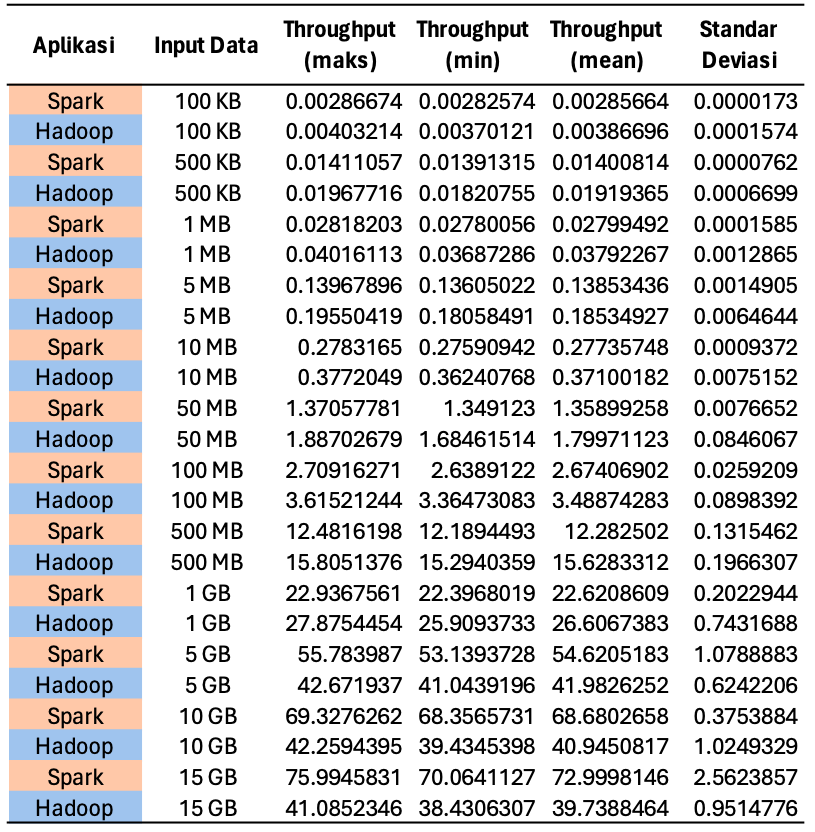
\includegraphics[width=0.6\textwidth]{figures/ch04/4-sort-th-table}
  \label{table:4-sort-th-table}
\end{table}

\newpage
Pada beban kerja \textit{word count} (Gambar \ref{fig:throughput-wordcount}), Spark mencapai \textit{throughput} yang lebih tinggi daripada Hadoop. Perbedaan \textit{throughput} paling mencolok terlihat pada ukuran data terbesar (15 GB), dimana Spark mencapai \textit{throughput} lebih dari 120 MB/s, sedangkan Hadoop hanya mencapai sekitar 20 MB/s. Meskipun Spark menunjukkan peningkatan \textit{throughput} yang signifikan pada ukuran data besar (1 GB, 5 GB, 10 GB, dan 15 GB), pada data input yang lebih kecil, 100 KB sampai 100 MB, perbedaan \textit{throughput} antara Hadoop dan Spark tidak berbeda jauh untuk \textit{word count}.

\begin{figure}[h]
    \centering
    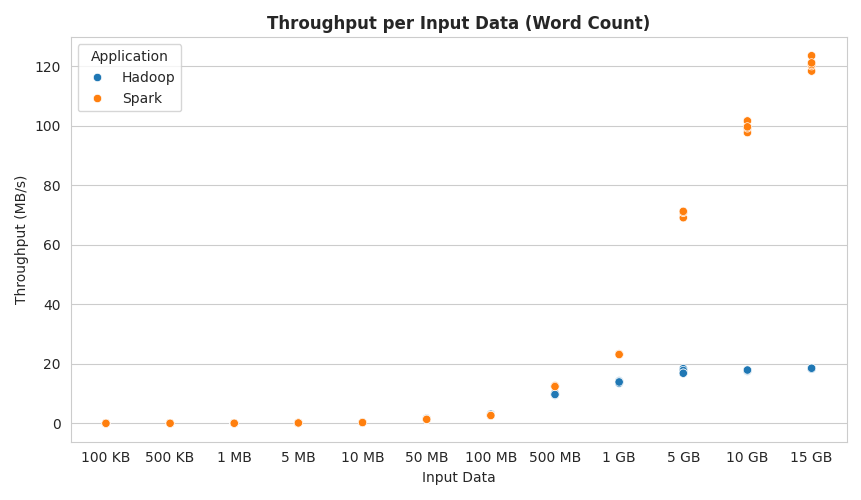
\includegraphics[width=0.8\textwidth]{figures/ch04/1-throughput-wordcount.png}
    \caption{Persebaran \textit{Throughput Word Count} (Hadoop, Spark)}
    \label{fig:throughput-wordcount}
\end{figure}


Tabel \ref{table:4-wc-th-table} menunjukkan data yang lebih rinci mengenai \textit{throughput} \textit{word count} untuk Hadoop dan Spark. Berdasarkan tabel tersebut, terlihat bahwa Hadoop memiliki \textit{throughput} yang lebih rendah dibandingkan Spark, terutama pada ukuran data yang lebih besar.
Perbedaan kinerja ini dapat dilihat dari kolom "Throughput (maks)" dan "Throughput (min)". Misalnya, untuk input data 100 KB, Hadoop memiliki \textit{throughput} maksimum 0.00384808 MB/s, sedangkan Spark memiliki \textit{throughput} maksimum 0.00286102 MB/s. Ketika input data mencapai 10 GB, \textit{throughput} maksimum Hadoop mencapai 17.9153442 MB/s, sementara Spark mencapai 101.596455 MB/s.

\begin{table}[h]
  \centering
  \caption{Statistika Deskriptif \textit{Throughput} (\textit{Word Count})}
  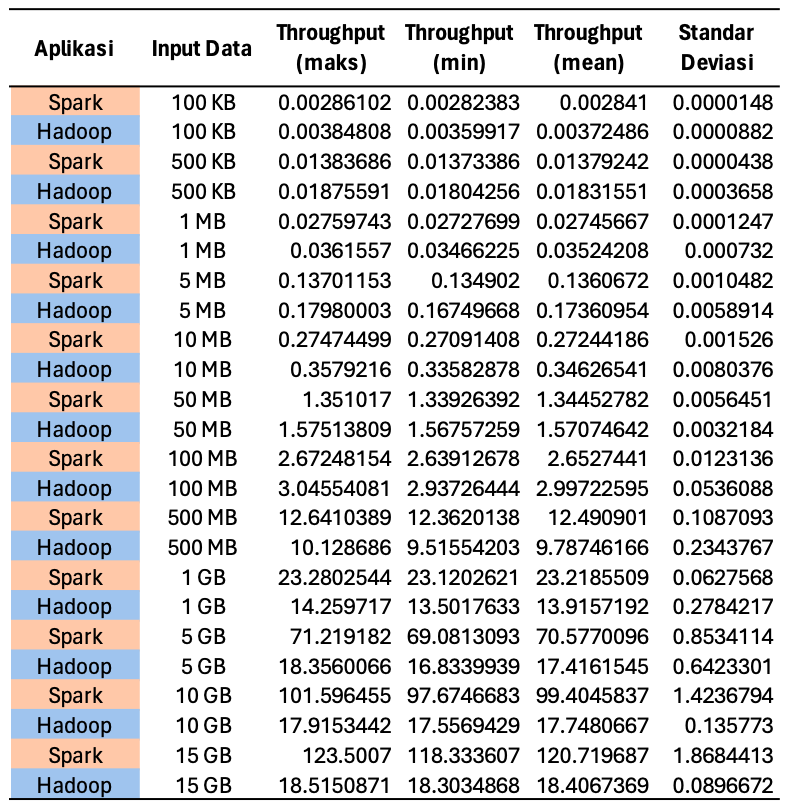
\includegraphics[width=0.6\textwidth]{figures/ch04/4-wc-th-table}
  \label{table:4-wc-th-table}
\end{table}

Hasil ini menunjukkan bahwa Spark lebih unggul dalam menangani data berukuran besar untuk kedua tugas pemrosesan data tersebut. Spark mampu mempertahankan \textit{throughput} yang lebih tinggi dibandingkan Hadoop, terutama saat menangani data berukuran besar, dengan rincian sebagai berikut:
\begin{enumerate}
\item Untuk beban kerja \textit{sort}, Spark lebih unggul pada ukuran data 1 GB, 5 GB, 10 GB, dan 15 GB.
\item Untuk beban kerja \textit{word count}, Spark lebih unggul pada ukuran data 1 GB, 5 GB, 10 GB, dan 15 GB.
\end{enumerate}

Secara keseluruhan, Spark menunjukkan kinerja yang lebih baik dalam hal \textit{throughput} terutama pada data berukuran besar, sementara Hadoop masih menunjukkan performa yang kompetitif pada data berukuran kecil hingga menengah.

\newpage
\section{Analisis dan Evaluasi Hasil Eksperimen: Penggunaan Sumber Daya}
\subsection{Penggunaan CPU}
Gambar \ref{fig:4-penggunaan-cpu-all-sort} dan Gambar \ref{fig:4-penggunaan-cpu-all-wordcount} menunjukkan pola penggunaan CPU oleh Hadoop dan Spark untuk beban kerja \textit{sort} dan \textit{word count} pada berbagai ukuran data. Sumbu x mewakili waktu dalam detik, sedangkan sumbu y mewakili persentase penggunaan CPU. Setiap grafik menunjukkan ukuran data yang berbeda, mulai dari 100 KB hingga 15 GB. Titik hitam pada gambar menandakan titik perpotongan Hadoop dan Spark pada waktu yang sama. Titik hitam tersebut berfungsi sebagai batas kondisi dimana penggunaan CPU Hadoop lebih tinggi dibandingkan Spark atau sebaliknya. Selanjutnya, titik hitam ini akan memberikan informasi visual mengenai perubahan dominasi penggunaan CPU antara Hadoop dan Spark selama proses komputasi.

Tabel \ref{fig:4-state-sort} dan Tabel \ref{fig:4-state-wordcount} menunjukkan perbandingan \textit{state} penggunaan CPU antara Hadoop ($U_h$) dan Spark ($U_s$) pada beban kerja \textit{sort} dan \textit{word count}. \textit{State} $U_h > U_s$ menunjukkan durasi waktu di mana penggunaan CPU Hadoop lebih tinggi daripada Spark, sementara \textit{state} $U_h < U_s$ menunjukkan sebaliknya.

Pada beban kerja \textit{sort} seperti yang terlihat pada Gambar \ref{fig:4-penggunaan-cpu-all-sort}, perbedaan pola penggunaan CPU antara Hadoop dan Spark terlihat pada ukuran data yang lebih besar. Jika dilihat pada input data 100 KB hingga 1 GB, penggunaan CPU pada masing-masing Hadoop dan Spark tidak terlihat perbedaannya. Selanjutnya, pada input data 5 GB, 10 GB, dan 15 GB, penggunaan CPU Hadoop sangat fluktuatif berkisar pada 60\% sampai 95\% pada dua per tiga bagian waktu awal eksekusi, dan satu per tiga waktu akhir eksekusi mengalami penurunan yang berkisar pada 20\% sampai 80\%. Berbeda dengan Hadoop, Spark memiliki penggunaan CPU yang lebih stabil, yaitu terkadang pada 60\% sampai 80\%, dan terkadang juga pada 80\% sampai 100\%).

Pada Tabel \ref{fig:4-state-sort}, terlihat bahwa durasi \textit{state} $U_h > U_s$ secara konsisten lebih tinggi dibandingkan dengan $U_h < U_s$ pada semua ukuran data. Hal ini menunjukkan bahwa Hadoop menggunakan lebih banyak CPU dibandingkan Spark untuk beban kerja \textit{sort}. Ketika ukuran data meningkat, perbedaan antara $U_h > U_s$ dan $U_h < U_s$ semakin besar. Hal ini menunjukkan bahwa Hadoop semakin intensif dalam penggunaan CPU dibandingkan Spark seiring dengan bertambahnya ukuran data.

\begin{table}[h]
  \centering
  \caption{Perbandingan \textit{State (Sort)}}
  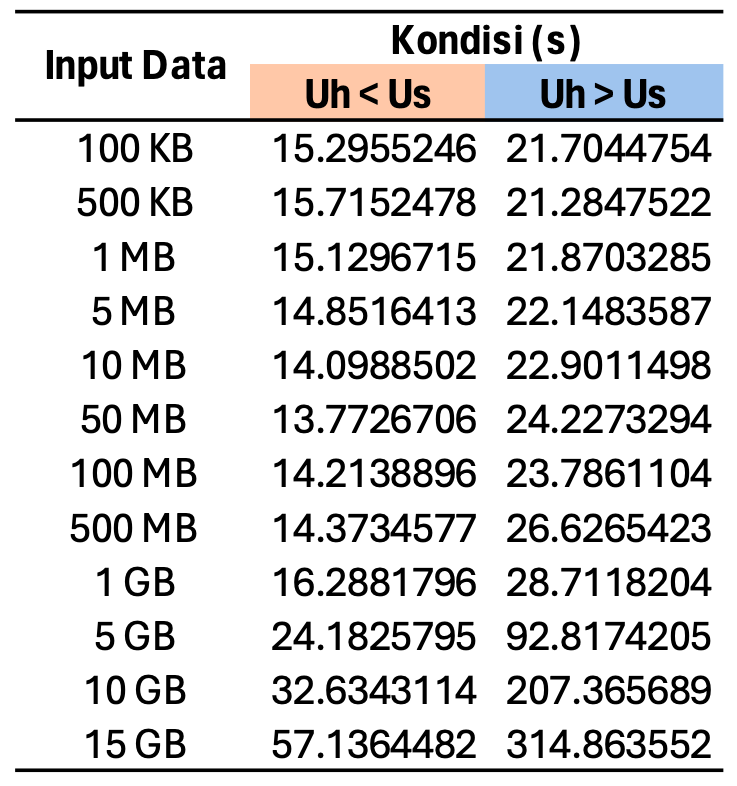
\includegraphics[width=0.45\textwidth]{figures/ch04/4-kondisi-sort}
  \label{fig:4-state-sort}
\end{table}

Pada beban kerja \textit{word count} seperti yang terlihat pada Gambar \ref{fig:4-penggunaan-cpu-all-wordcount}, Hadoop menunjukkan penggunaan CPU yang lebih fluktuatif (naik turun) dan tinggi secara keseluruhan dibandingkan dengan Spark. Penggunaan CPU pada waktu ke-0 hingga ke-10 pada Hadoop berkisar pada 10\% sampai 60\%. Setelah itu, penggunaan CPU Hadoop naik sampai ke 100\% dan naik turun. Jika dilihat dari input data yang lebih besar yaitu 15 GB, Hadoop memiliki pola CPU yang hampir sama pada setiap data input, yaitu 
\begin{enumerate}
\item Sepuluh detik pertama penggunaan CPU berada pada 10\% sampai 60\%
\item Setengah waktu eksekusi naik turun pada penggunaan CPU 60\% hingga 100\%
\item Setengah waktu eksekusi terakhir menurunkan penggunaan CPU pada 50\% sampai 90\%
\end{enumerate}
Selanjutnya, Spark juga memiliki pola tersendiri. Penggunaan CPU Spark pada detik pertama sampai detik ke lima belas fluktuatif pada 20\% hingga 50\%. Pada waktu ke-16 sampai waktu ke-35 turun hingga 0\%, dan naik kembali pada waktu ke-35. Hal yang menarik lainnya adalah penggunaan CPU Spark tidak menyentuh 100\%, tetapi memiliki waktu eksekusi beban kerja yang lebih cepat pada \textit{word count}.

Pada Tabel \ref{fig:4-state-wordcount}, variasi dalam perbandingan \textit{state} \textit{word count} lebih terlihat dibandingkan  \textit{sort}. Secara umum, durasi \textit{state} $U_h > U_s$ tetap lebih tinggi dibandingkan $U_h < U_s$. Pada beban kerja \textit{word count}, durasi $U_h < U_s$ tidak menunjukkan pola yang konsisten dengan ukuran data, tetapi durasi $U_h > U_s$ cenderung meningkat seiring dengan bertambahnya ukuran data. Ini menunjukkan bahwa Hadoop lebih sering mengalami penggunaan CPU yang lebih tinggi dibandingkan Spark, terutama pada ukuran data yang lebih besar.

\begin{table}[h]
  \centering
  \caption{Perbandingan \textit{State  (Word Count)}}
  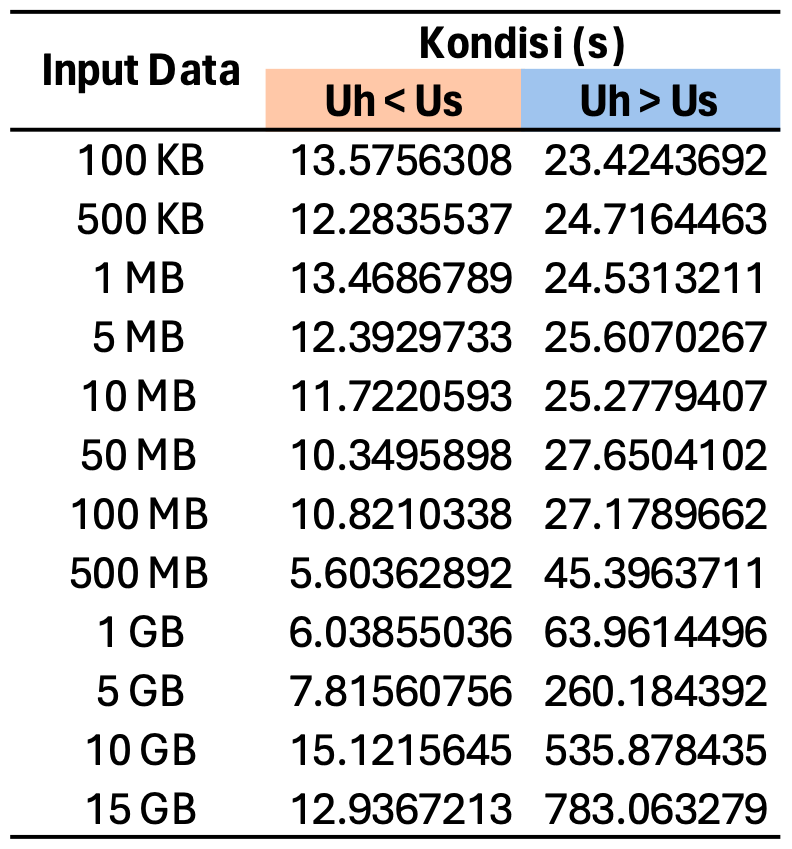
\includegraphics[width=0.45\textwidth]{figures/ch04/4-kondisi-wc}
  \label{fig:4-state-wordcount}
\end{table}

\newpage
Pada kedua tugas, terlihat bahwa beban kerja \textit{word count} cenderung menunjukkan pola penggunaan CPU yang lebih tinggi dan konsisten dibandingkan dengan beban kerja \textit{sort}. Pada beban kerja \textit{word count}, umumnya penggunaan CPU Hadoop lebih tinggi dan merata di sepanjang waktu eksekusi jika dibandingkan dengan Spark. Di sisi lain, beban kerja \textit{sort} menunjukkan penggunaan CPU yang cenderung lebih fluktuatif, dengan periode lonjakan dan penurunan yang signifikan, baik pada Hadoop maupun Spark.

Secara keseluruhan, Hadoop cenderung menggunakan CPU dengan lebih intensif dan fluktuatif dibandingkan Spark, terutama pada tugas \textit{word count}. Spark, meskipun tidak selalu menggunakan CPU hingga 100\%, mampu menyelesaikan tugas dengan waktu eksekusi yang lebih cepat, menunjukkan efisiensi penggunaan sumber daya yang lebih baik.

\begin{landscape}
\begin{figure}[h]
    \centering
    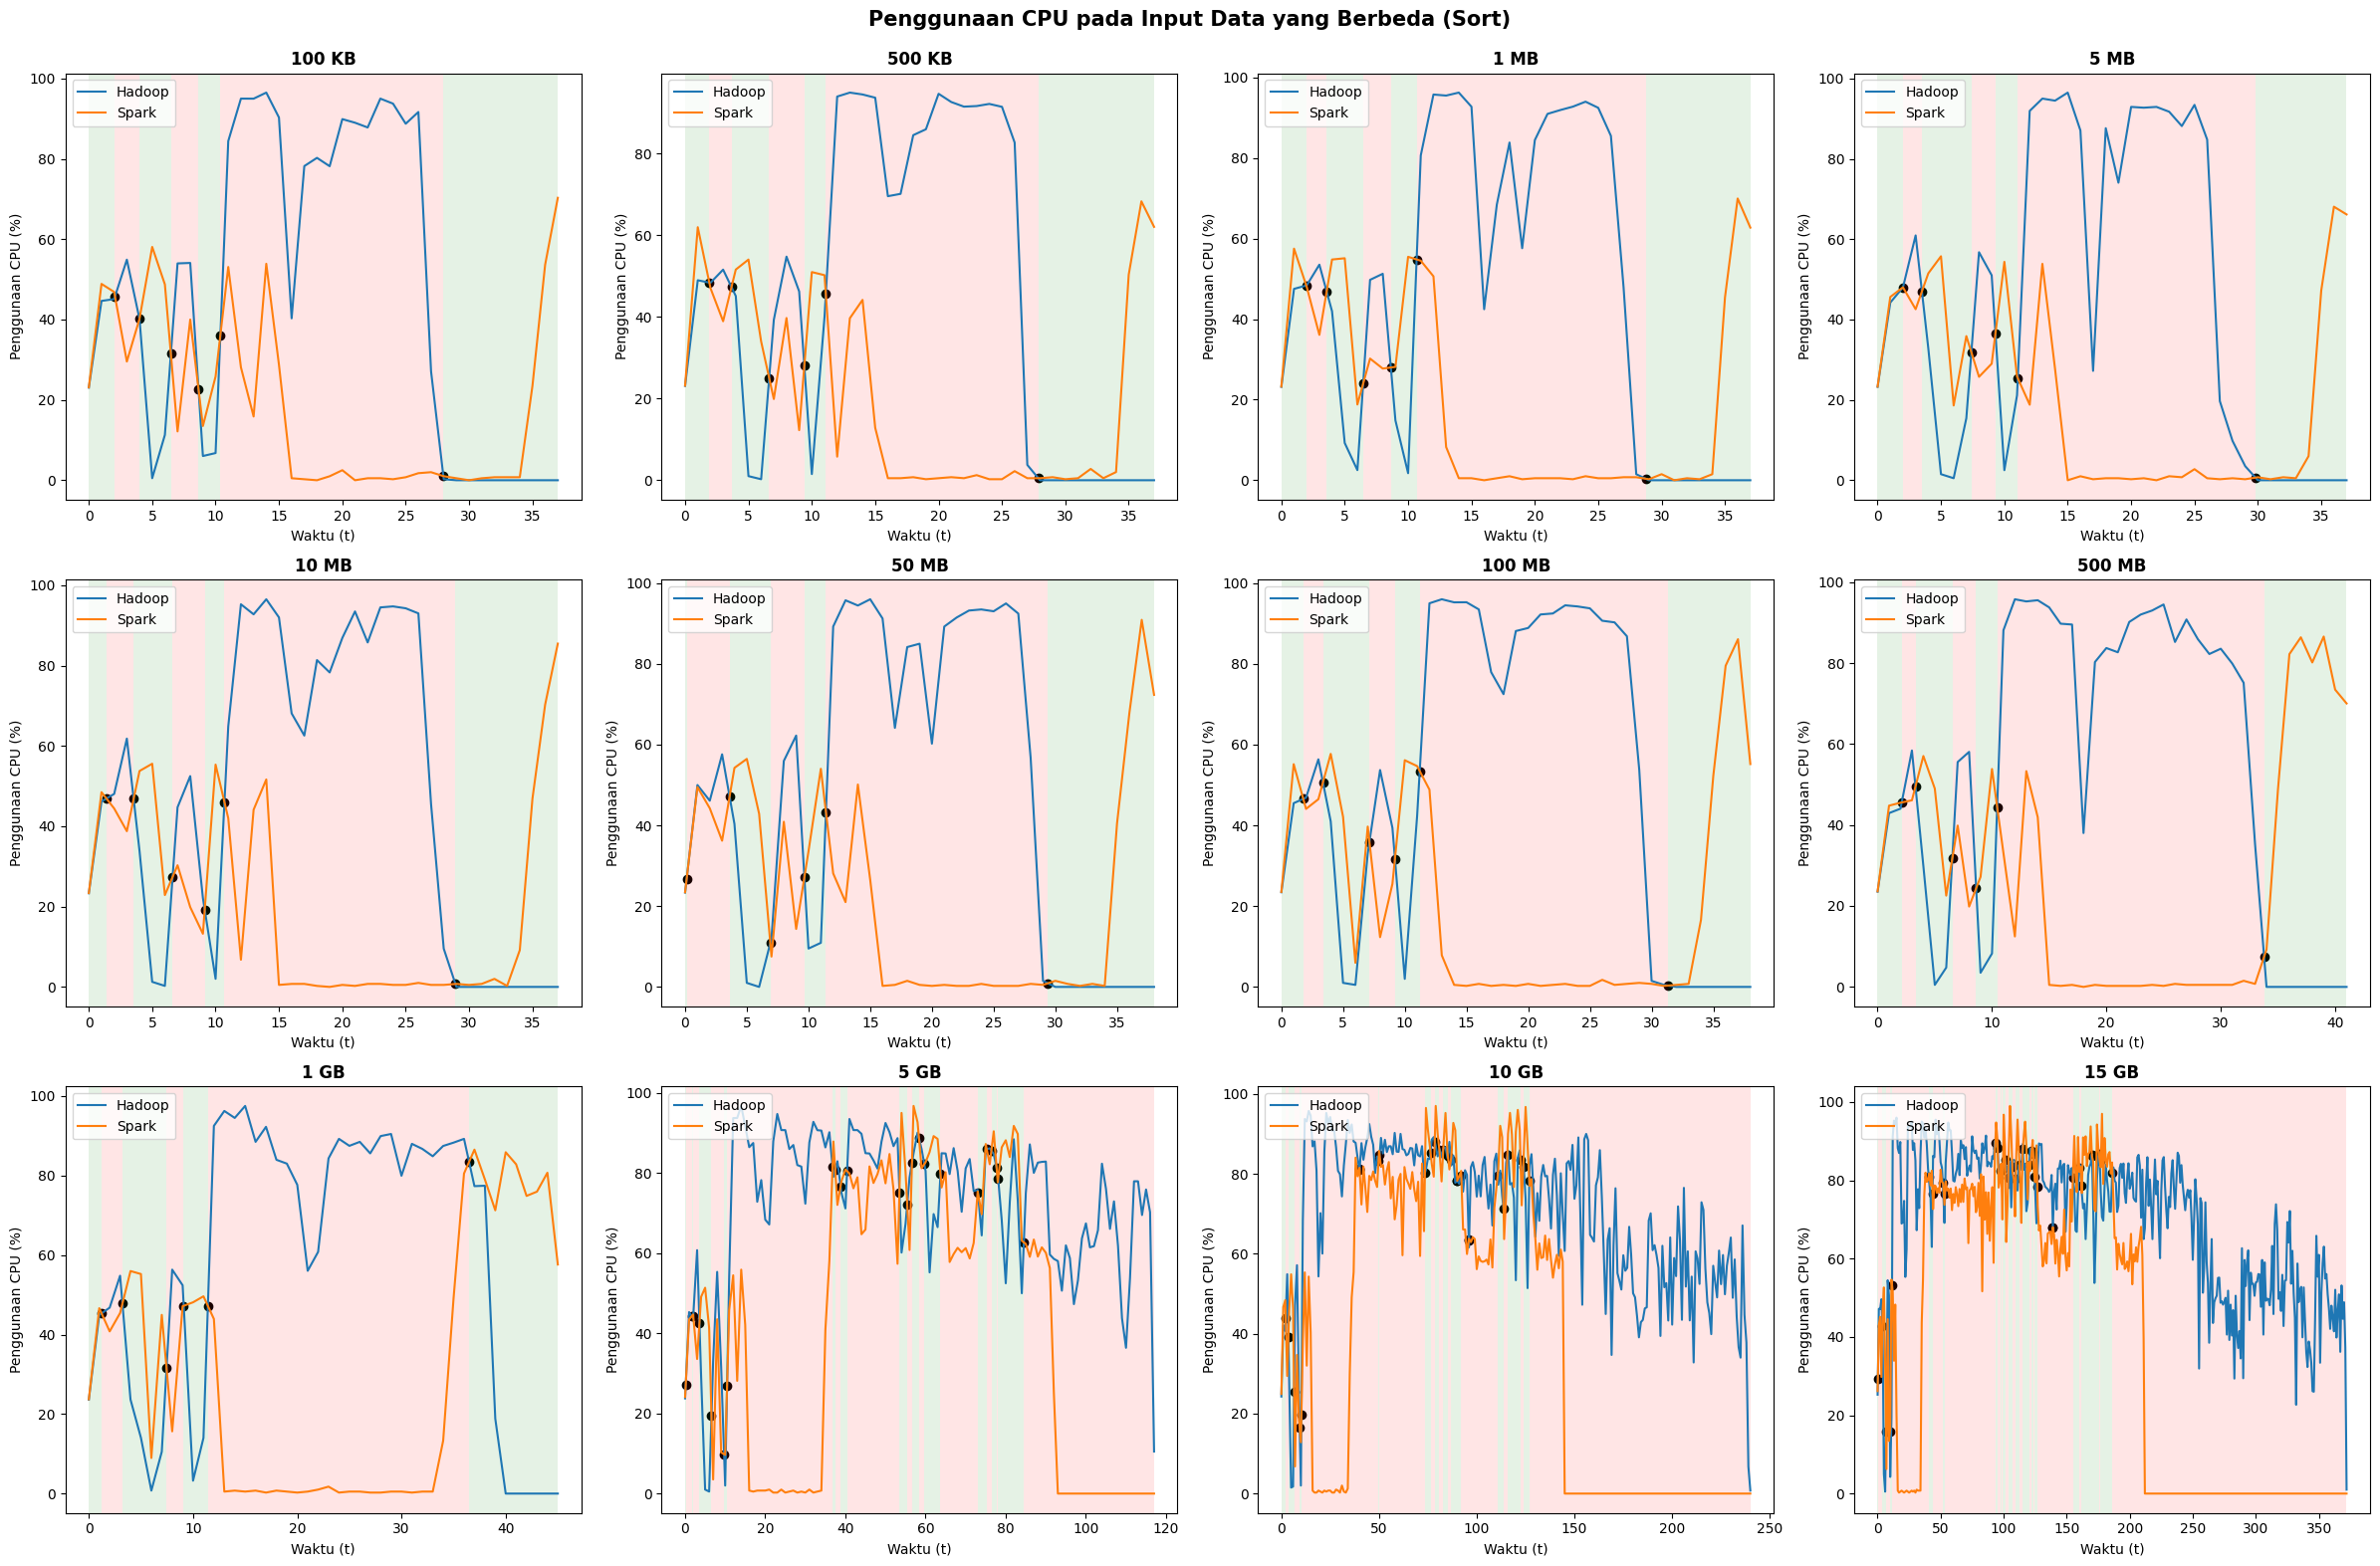
\includegraphics[height=0.6\linewidth]{figures/ch04/4-penggunaan-cpu-all-sort.png}
    \caption{Penggunaan CPU (\textit{Sort})}
    \label{fig:4-penggunaan-cpu-all-sort}
\end{figure}
\end{landscape}

\begin{landscape}
\begin{figure}[h]
    \centering
    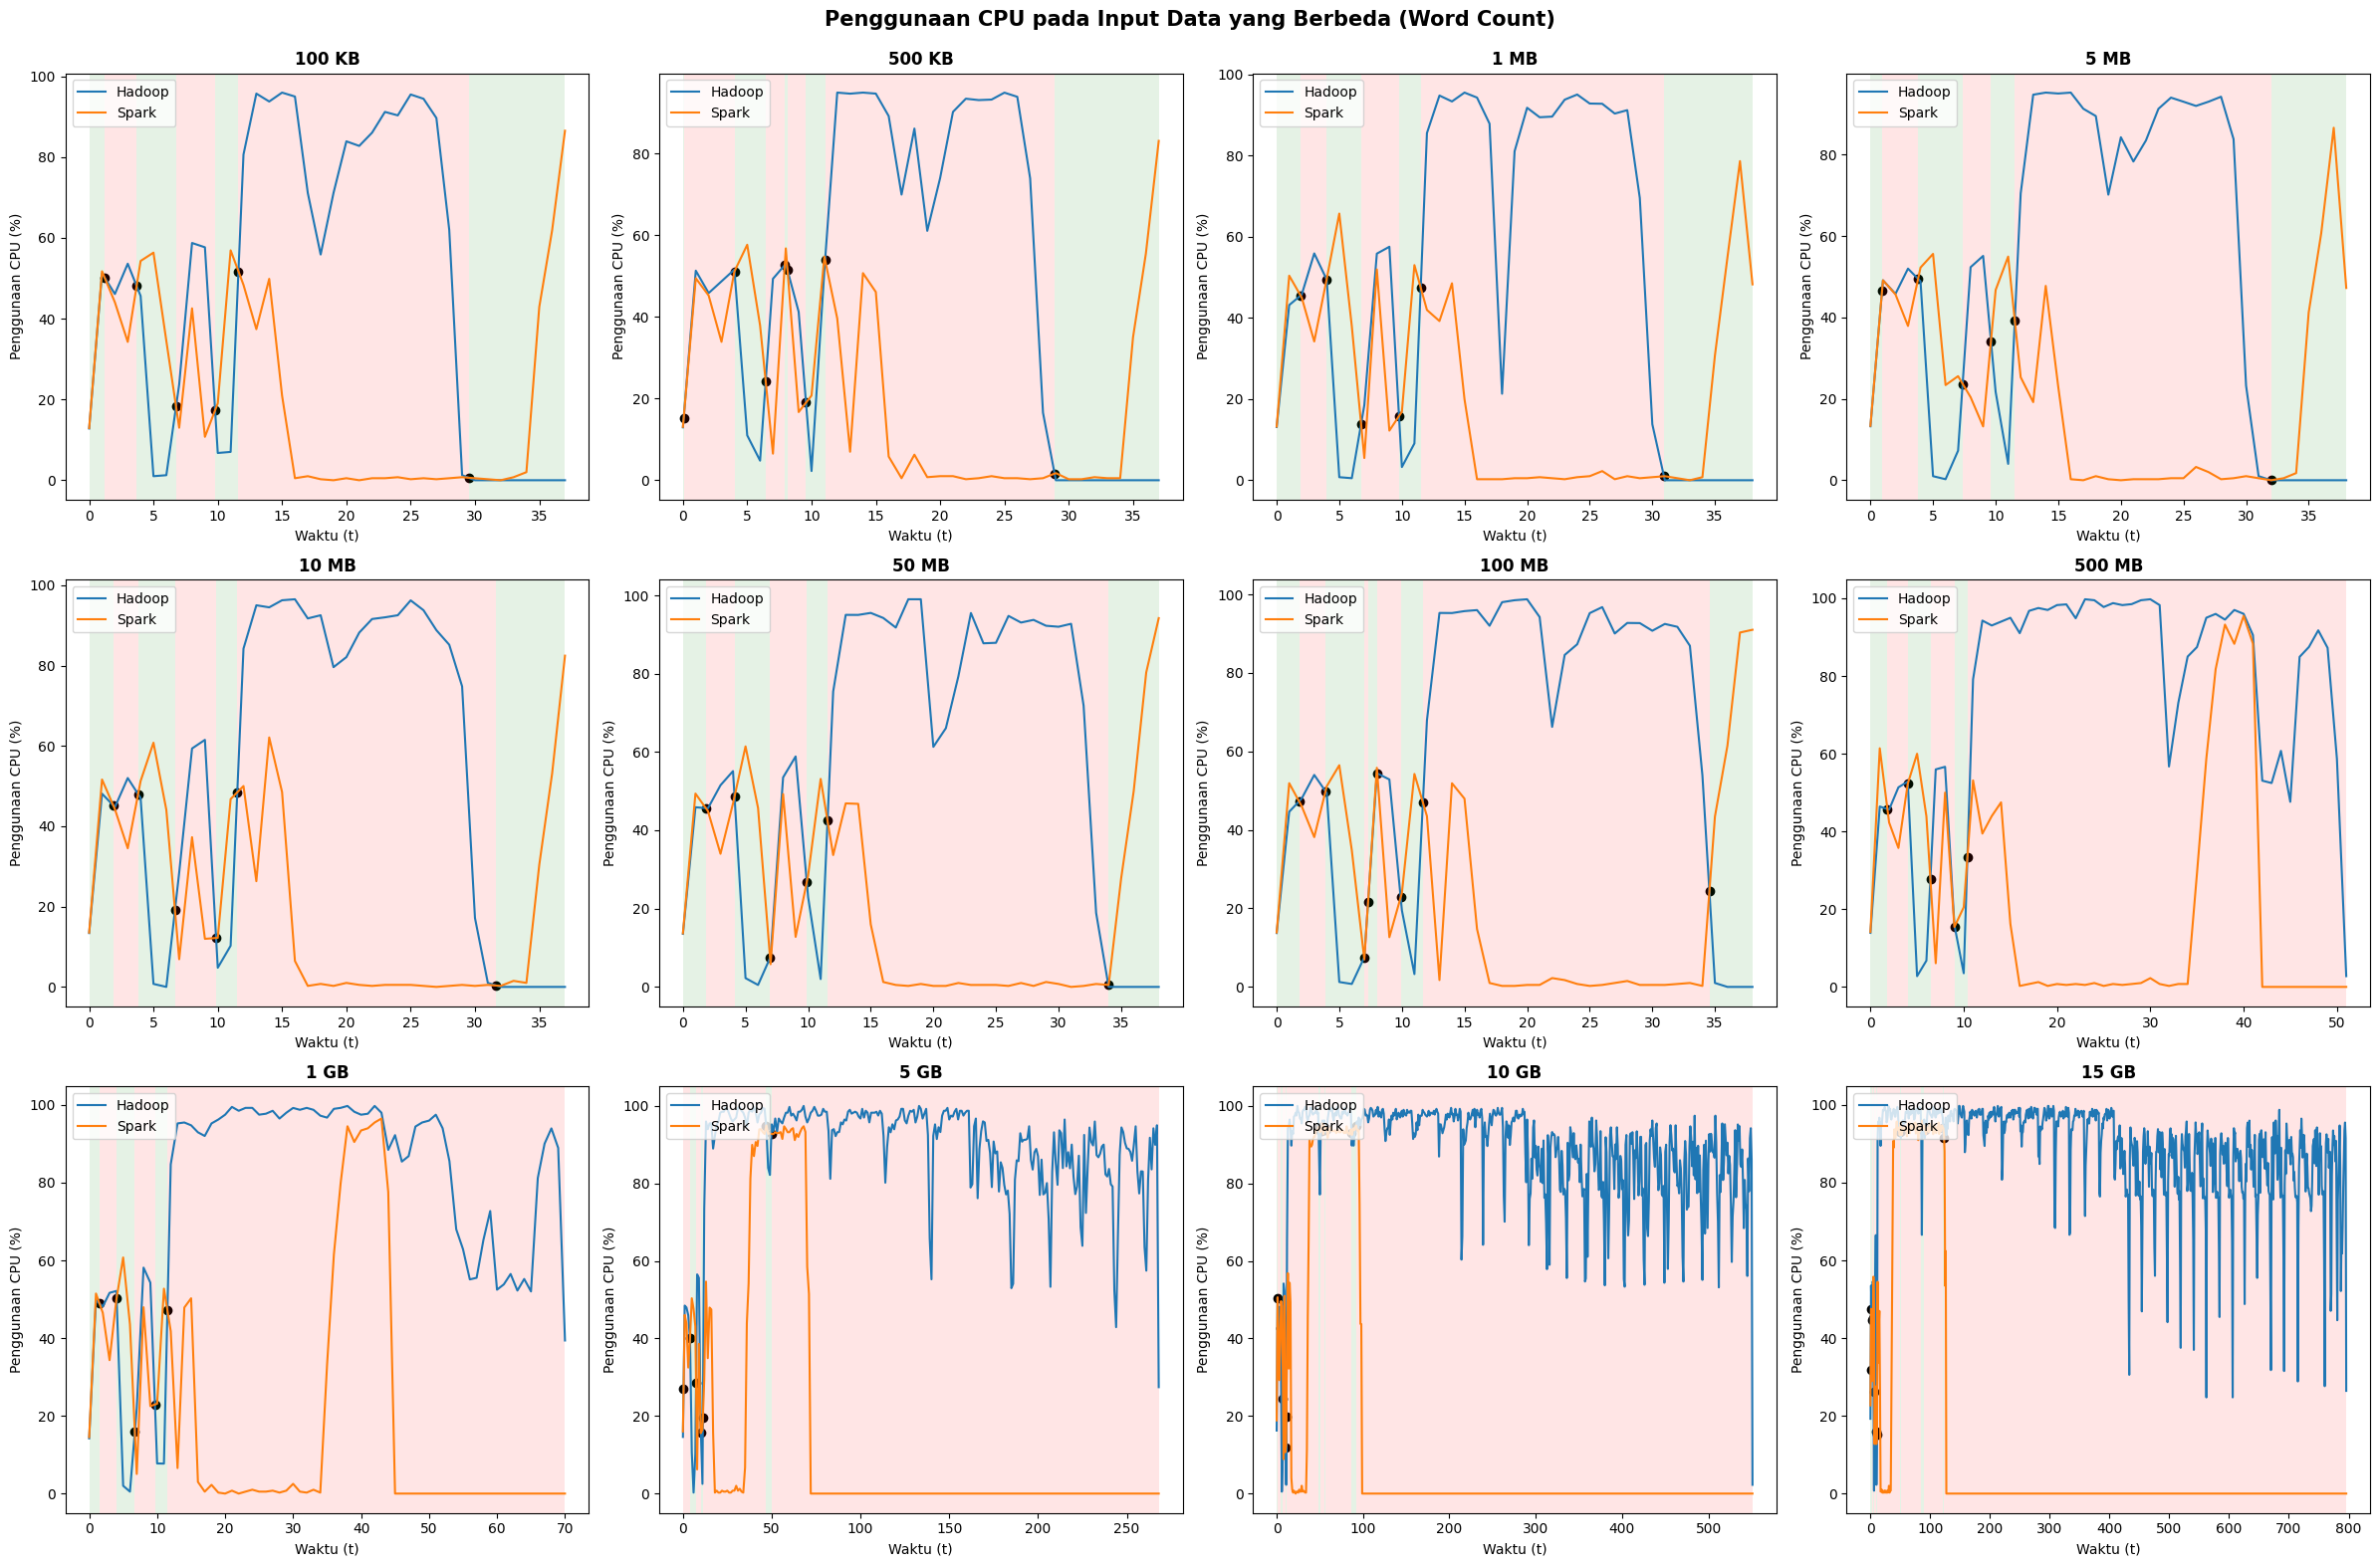
\includegraphics[height=0.6\linewidth]{figures/ch04/4-penggunaan-cpu-all-wordcount.png}
    \caption{Penggunaan CPU (\textit{Word Count})}
    \label{fig:4-penggunaan-cpu-all-wordcount}
\end{figure}
\end{landscape}

\subsection{Utilisasi Sistem}
Setiap gambar akan terdiri dari dua baris dan tiga kolom. Baris pertama berisi visualisasi utilisasi sistem untuk Hadoop dan baris kedua berisi visualisasi untuk Spark. Setiap baris berisi tiga utilisasi sistem, Penggunaan CPU (\%), \textit{Disk} I/O (MB), Memori (GB).

Berdasarkan analisis pola penggunaan CPU pada tahap sebelumnya yang menunjukkan bahwa penggunaan CPU Hadoop dan Spark memiliki polanya masing-masing, maka pada tahap ini hanya akan ditampilkan utilisasi sistem pada input data terbesar (15 GB).

Pada beban kerja \textit{sort} dan input data terbesar, yaitu 15 GB (seperti yang ditunjukkan pada Gambar \ref{fig:5-util-sistem-sort-fiveteengig}), utilisasi sistem pada Hadoop dan Spark terlihat jelas perbedaannya. Jika dilihat pada penggunaan CPU, Hadoop membutuhkan waktu penggunaan CPU yang lebih lama, yaitu sekitar 370 detik, dimana Spark hanya membutuhkan waktu sekitar 220 detik. Selanjutnya, Hadoop memiliki penggunaan CPU "\textit{user}" yang lebih stabil, jika dibandingkan dengan Spark yang naik turun secara konstan. Penggunaan CPU "\textit{wait}" akan naik ketika penggunaan CPU "\textit{user}" turun. Bergeser pada \textit{disk I/O}, Hadoop memiliki siklus baca tulis yang lebih intensif jika dibandingkan pada Spark. Selanjutnya, jika dilihat dari penggunaan memori, Spark lebih "rakus" akan memori. Hal ini ditandai dengan puncaknya membutuhkan memori sekitar 6 hingga 7 GB, dimana Hadoop hanya membutuhkan memori sekitar 3.5 GB.

\begin{figure}[h]
    \centering
    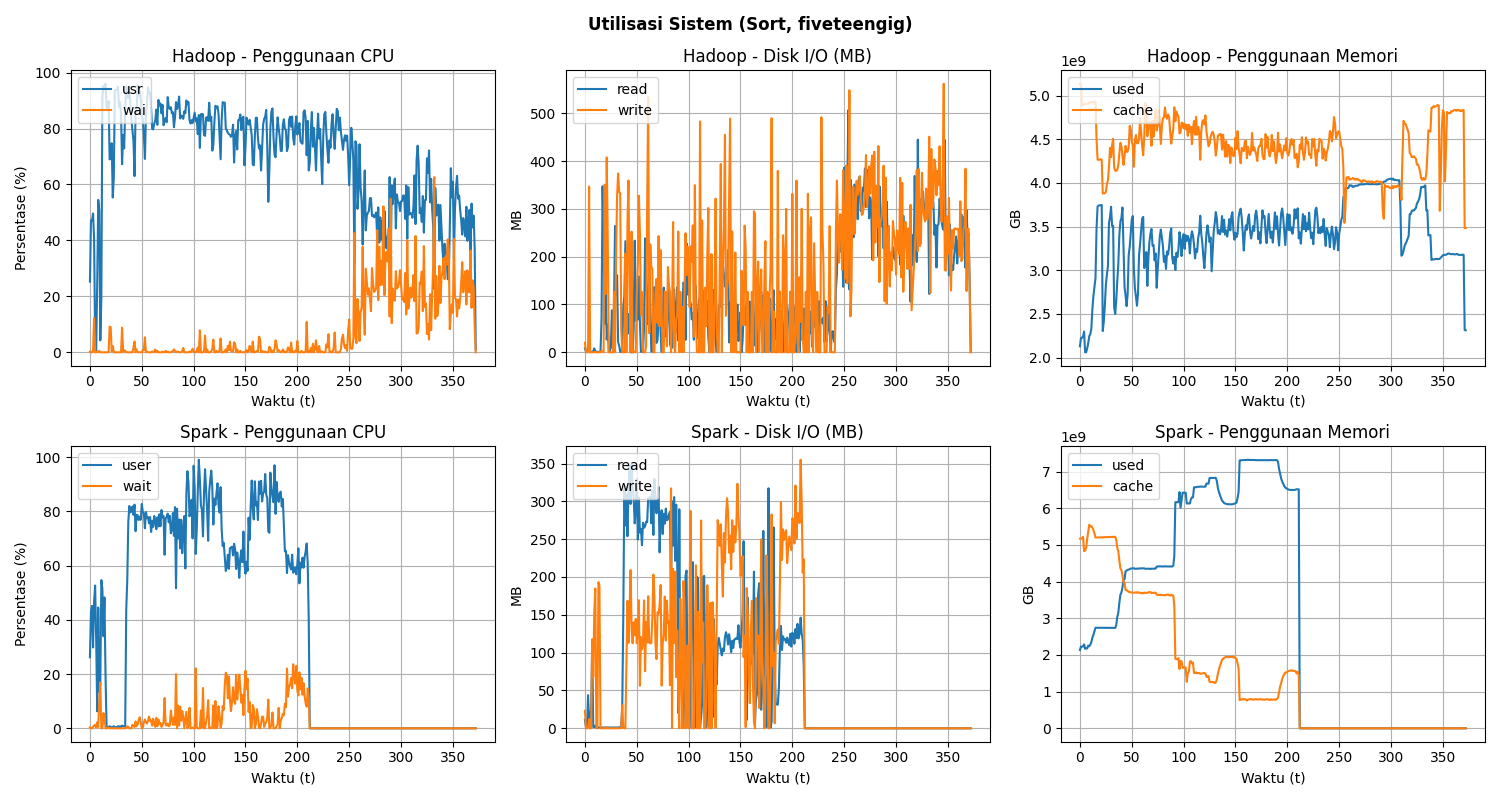
\includegraphics[width=0.85\textwidth]{figures/ch04/5-util-sistem-sort-fiveteengig}
    \caption{Utilisasi Sistem (\textit{Sort}) pada Input Data 15 GB}
    \label{fig:5-util-sistem-sort-fiveteengig}
\end{figure}

Pada beban kerja \textit{word count} dan input data terbesar, yaitu 15 GB (seperti yang ditunjukkan pada Gambar \ref{fig:5-util-sistem-wordcount-fiveteengig}), utilisasi sistem pada Hadoop dan Spark terlihat jelas perbedaannya. Pada penggunaan CPU, Hadoop memiliki aktivitas penggunaan yang lebih tinggi dan lebih konstan sampai akhir waktu eksekusi. Hal ini berbeda dengan Spark yang hanya butuh waktu sekitar 150 detik saja dengan penggunaan CPU yang hanya 90\%. Selanjutnya, pada aktivitas baca tulis (\textit{disk I/O}), Hadoop memiliki aktivitas baca yang lebih intensif (sepanjang waktu eksekusi) dengan sedikit aktivitas tulis (pada awal waktu eksekusi). Aktivitas baca yang dilakukan oleh Hadoop berada pada ukuran 50 hingga 100 MB setiap waktunya. Pada Spark, aktivitas baca tersebut berukuran 150 hingga 200 MB. Kemudian, jika ditinjau melalui penggunaan memori, memori yang dibutuhkan Hadoop berkisar pada 2.5 hingga 3.7 GB. Pada Spark, memori yang dibutuhkan berkisar pada 2 hingga 4.5 GB.  

\begin{figure}[h]
    \centering
    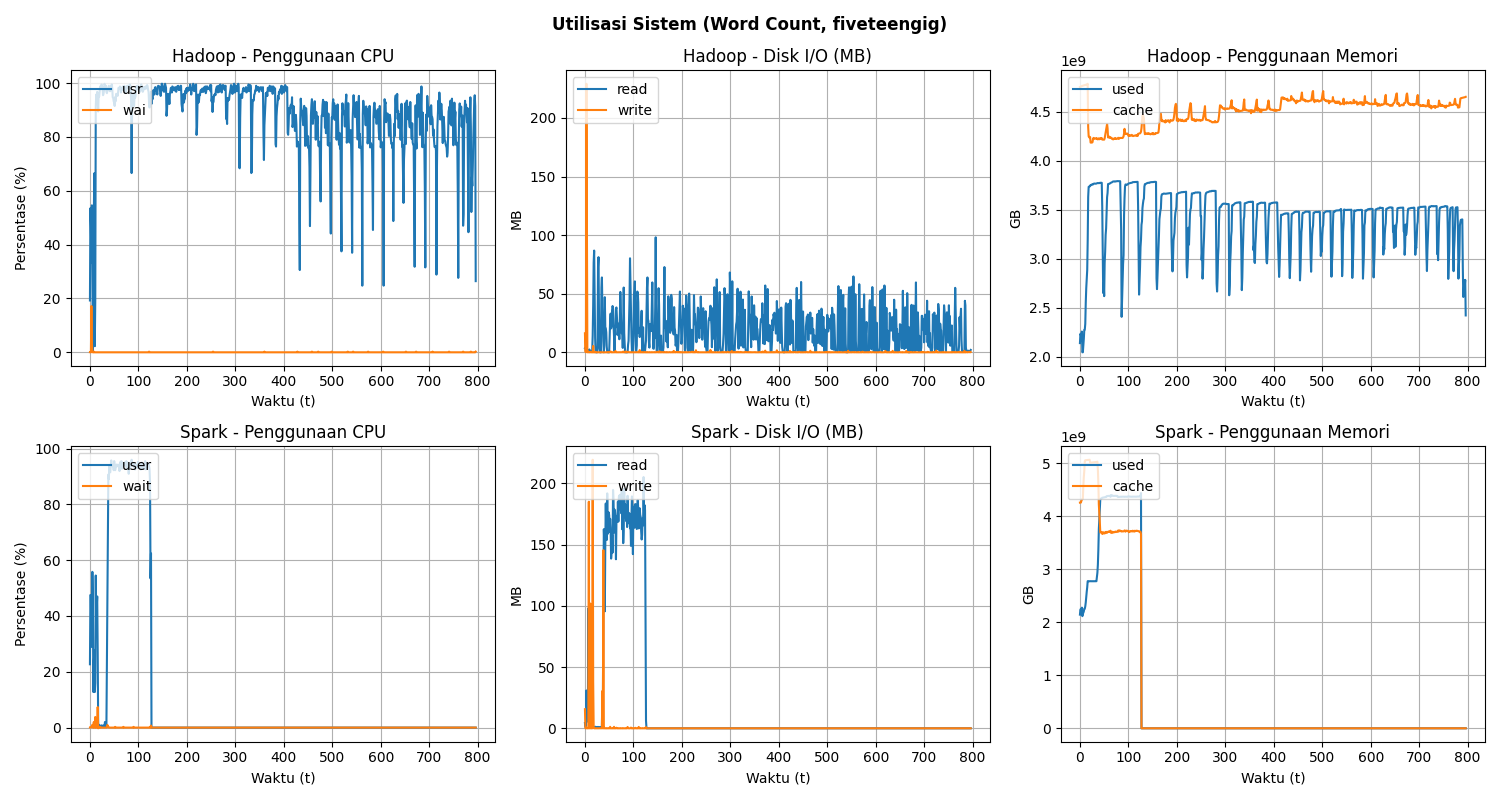
\includegraphics[width=0.85\textwidth]{figures/ch04/5-util-sistem-wordcount-fiveteengig}
    \caption{Utilisasi Sistem (\textit{Word Count}) pada Input Data 15 GB}
    \label{fig:5-util-sistem-wordcount-fiveteengig}
\end{figure}

Hadoop menunjukkan aktivitas \textit{Disk} I/O yang jauh lebih tinggi dibandingkan dengan Spark, terutama pada beban kerja \textit{sort}. Grafik \textit{Disk} I/O Hadoop menunjukkan lonjakan aktivitas baca dan tulis yang signifikan sepanjang waktu eksekusi. Hal ini sesuai dengan pendekatan berbasis \textit{disk} Hadoop yang membutuhkan pembacaan dan penulisan data ke \textit{disk} secara intensif. Sebaliknya, Spark, dengan arsitektur \textit{in-memory}, meminimalkan operasi \textit{Disk} I/O. Grafik \textit{Disk} I/O Spark menunjukkan aktivitas yang jauh lebih rendah dan stabil, yang berkontribusi pada peningkatan performanya.

Spark menunjukkan penggunaan memori yang lebih tinggi dan stabil dibandingkan dengan Hadoop, terutama pada beban kerja \textit{sort}. Grafik penggunaan memori Spark menunjukkan garis yang cenderung mendatar pada tingkat utilisasi yang tinggi, menunjukkan bahwa Spark menyimpan data dalam RAM untuk akses yang lebih cepat dan pemrosesan yang efisien. Penggunaan memori Hadoop lebih rendah dan fluktuatif, menunjukkan bahwa Hadoop tidak memanfaatkan memori secara optimal. 

\section{Perbandingan dengan Penelitian Sebelumnya \cite{samadiPerformanceComparisonHadoop2018}}
Penelitian terdahulu yang telah dilakukan oleh Yassir Samadi, dkk. mendapatkan hasil seperti pada Tabel \ref{table:penelitian-lama}. Pada gambar tersebut terlihat bahwa pada input data 1 GB dan pada beban kerja \textit{word count}, terjadi peningkatan performa sebesar 2.92, pada input data 5 GB sebesar 3.64, dan begitu juga pada input data 10 GB sebesar 3.52.

%\begin{figure}[h]
%    \centering
%    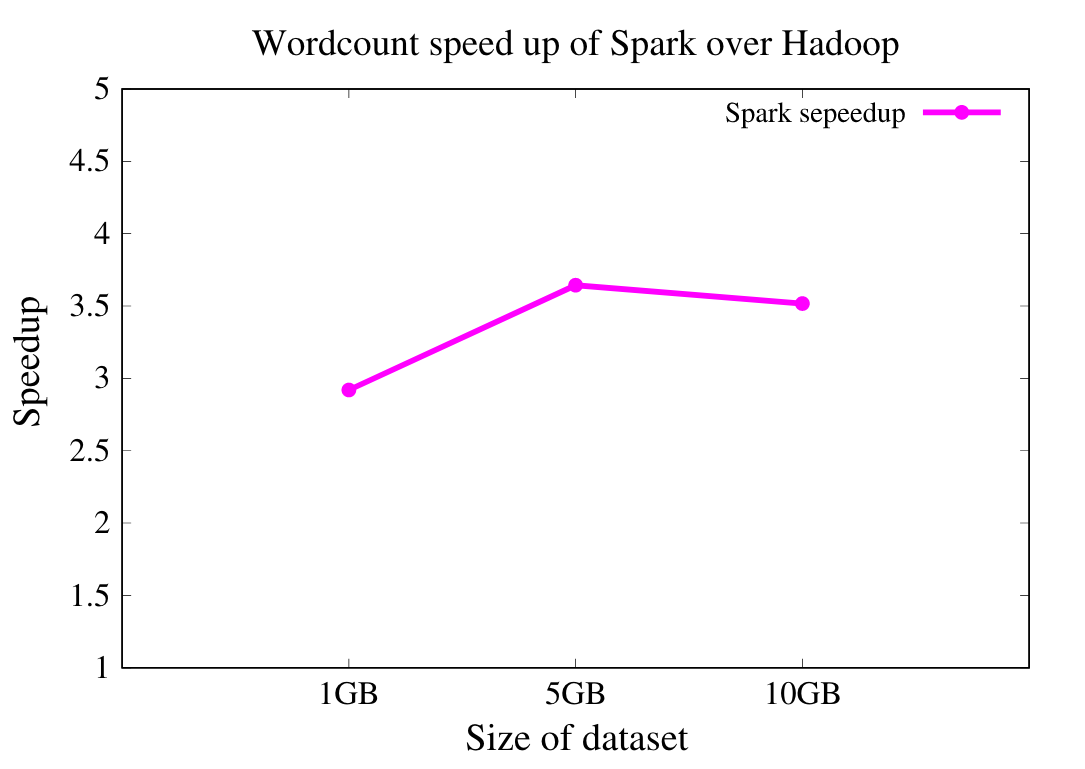
\includegraphics[width=1\textwidth]{figures/ch04/0-penelitian lama}
%    \caption{Rasio Peningkatan Performa Spark-Hadoop Berdasarkan Input Data \cite{samadiPerformanceComparisonHadoop2018}}
%    \label{fig:0-penelitian-lama}
%\end{figure}

\begin{table}[h]
  \centering
  \caption{Rasio Peningkatan Performa Spark-Hadoop \cite{samadiPerformanceComparisonHadoop2018}}
  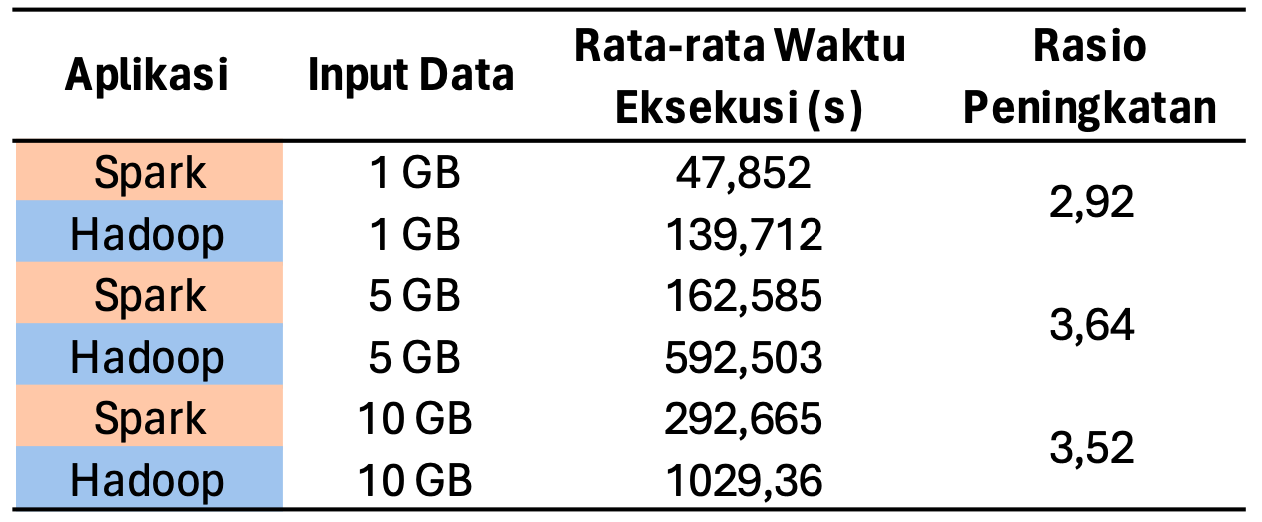
\includegraphics[width=0.6\textwidth]{figures/ch04/0-penelitian-lama-new}
  \label{table:penelitian-lama}
\end{table}

Penelitian ini menghasilkan hasil yang serupa, seperti yang ditunjukkan pada Tabel \ref{table:penelitian-baru}. Pada penelitian ini, rasio peningkatan performa naik secara bertahap dari input data 1 GB, 5 GB, 10 GB, hingga 15 GB. Hal ini dapat terjadi karena adanya perbedaan konfigurasi perangkat keras dan perbedaan versi perangkat lunak yang digunakan.

\begin{table}[h]
  \centering
  \caption{Rasio Peningkatan Performa Spark-Hadoop}
  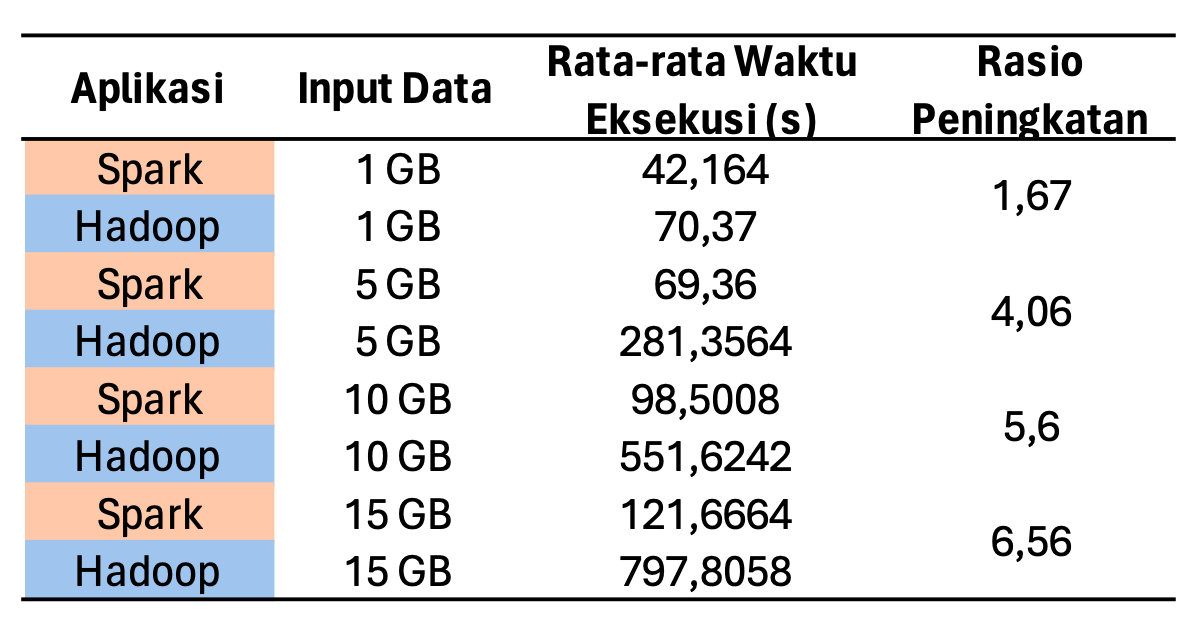
\includegraphics[width=0.6\textwidth]{figures/ch04/0-penelitian-baru}
  \label{table:penelitian-baru}
\end{table}

Pada Tabel \ref{table:penelitian-baru}, dapat dilihat bahwa Spark menunjukkan peningkatan performa yang signifikan dibandingkan Hadoop pada berbagai ukuran input data. Pada input data 1 GB, Spark memiliki rasio peningkatan sebesar 1.67 kali lipat dibandingkan Hadoop. Pada input data 5 GB, rasio peningkatan naik menjadi 4.06 kali lipat. Begitu juga dengan input data 10 GB dan 15 GB, rasio peningkatannya masing-masing sebesar 5.6 kali lipat dan 6.56 kali lipat.

%Secara keseluruhan, hasil penelitian ini konsisten dengan penelitian sebelumnya, namun menunjukkan peningkatan performa yang lebih signifikan pada ukuran data yang lebih besar. Hal ini menunjukkan bahwa Spark lebih efisien dalam menangani data dalam skala besar dibandingkan Hadoop, terutama pada beban kerja \textit{word count}.


